\documentclass[kdmile,a4paper]{kdmile}
\usepackage{graphicx,url}
\usepackage[T1]{fontenc}
\usepackage{booktabs}

\newtheorem{theorem}{Teorema}[section]
\newtheorem{conjecture}[theorem]{Conjectura}
\newtheorem{corollary}[theorem]{Corol\'{a}rio}
\newtheorem{proposition}[theorem]{Proposi\c{c}\~{a}o}
\newtheorem{lemma}[theorem]{Lema}
\newdef{definition}[theorem]{Defini\c{c}\~{a}o}
\newdef{remark}[theorem]{Observa\c{c}\~{a}o}

\markboth{N. M. R. da Silva and R. C. Pedrosa Silva}
{Trade-off between Privacy and Utility in Gradient Defenses under a Single-Client Protocol}

\title{Trade-off between Privacy and Utility in Gradient Defenses\\against Inversion Attacks under a Single-Client Protocol}

\author{Niege Marryany dos Reis da Silva\inst{1}, Rodrigo Cesar Pedrosa Silva\inst{1}}

\institute{Universidade Federal de Ouro Preto, Brazil \\ \email{niege.silva@aluno.ufop.edu.br} \\ \email{rodrigo.silva@ufop.edu.br}}

\begin{abstract}
Gradient inversion attacks reconstruct private training data from gradients shared in federated learning. Under a single-client factorial protocol spanning three image datasets, three architectures, five defense mechanisms and two batch sizes, differential privacy via DP-SGD yields the highest reconstruction error (mean MSE 0.865) but reduces test accuracy to 0.153, a 75\% drop relative to the undefended baseline. Random-$k$ sparsification at 10\% retention achieves the most favorable privacy--utility balance on CIFAR-10, raising MSE by up to 3.1-fold on Vision Transformers while preserving test accuracy within 0.3 percentage points on ViT (CNN incurs an $\approx$8\% drop). Top-$k$ sparsification at the same retention rate does not significantly increase reconstruction error against the iDLG attack ($p > 0.05$) and leaves label inference at 100\% accuracy. Defense effectiveness depends critically on dataset complexity, model architecture and compression parameters, limiting generalization from simple benchmarks such as MNIST.
\end{abstract}

\begin{CCSXML}
<ccs2012>
<concept>
<concept_id>10010147.10010257.10010293.10010294</concept_id>
<concept_desc>Computing methodologies~Neural networks</concept_desc>
<concept_significance>300</concept_significance>
</concept>
<concept>
<concept_id>10002978.10003022.10003023</concept_id>
<concept_desc>Security and privacy~Privacy-preserving protocols</concept_desc>
<concept_significance>500</concept_significance>
</concept>
<concept>
<concept_id>10010147.10010257.10010293.10010319</concept_id>
<concept_desc>Computing methodologies~Distributed artificial intelligence</concept_desc>
<concept_significance>300</concept_significance>
</concept>
</ccs2012>
\end{CCSXML}

\ccsdesc[300]{Computing methodologies~Neural networks}
\ccsdesc[500]{Security and privacy~Privacy-preserving protocols}
\ccsdesc[300]{Computing methodologies~Distributed artificial intelligence}

\keywords{differential privacy, federated learning, gradient compression, gradient inversion attacks, privacy and security in data mining}

\begin{document}

\begin{bottomstuff}
\end{bottomstuff}

\maketitle

% =============================================================================
% SE\c{C}\~{A}O 1 --- INTRODU\c{C}\~{A}O
% =============================================================================
\section{Introdu\c{c}\~{a}o}
\label{sec:introducao}

O aprendizado federado permite treinar modelos de aprendizado de m\'{a}quina a partir de dados distribuidos, sem centralizar amostras sens\'{i}veis \cite{McMahan2017}. Em cada rodada de treinamento, clientes calculam gradientes locais e os compartilham com um servidor agregador. Esse fluxo reduz a exposi\c{c}\~{a}o direta dos dados, mas n\~{a}o elimina riscos de privacidade. Ataques de invers\~{a}o de gradientes demonstram que informa\c{c}\~{o}es sobre amostras de treinamento podem ser reconstru\'{i}das a partir dos gradientes compartilhados \cite{Zhu2019,Geiping2020}.

Duas fam\'{i}lias de t\'{e}cnicas s\~{a}o frequentemente empregadas como mecanismos de defesa nesse contexto. A primeira baseia-se em privacidade diferencial, com destaque para m\'{e}todos que recortam gradientes e adicionam ru\'{\i}do gaussiano antes do compartilhamento \cite{Abadi2016}. A segunda emprega compress\~{a}o ou esparsifica\c{c}\~{a}o de gradientes, transmitindo apenas parte da informa\c{c}\~{a}o original por meio de t\'{e}cnicas como Top-$k$, Random-$k$ e quantiza\c{c}\~{a}o estoc\'{a}stica \cite{Stich2018,Wangni2018,Alistarh2017}. Essas abordagens reduzem o volume de comunica\c{c}\~{a}o e, em princ\'{\i}pio, limitam a quantidade de informa\c{c}\~{a}o dispon\'{\i}vel para reconstru\c{c}\~{a}o.

Apesar da diversidade de mecanismos descritos na literatura, compara\c{c}\~{o}es emp\'{\i}ricas sistem\'{a}ticas permanecem limitadas. Muitos estudos avaliam defesas de forma isolada, com datasets, arquiteturas ou protocolos de ataque distintos. A aus\^{e}ncia de um protocolo experimental comum dificulta a identifica\c{c}\~{a}o de configura\c{c}\~{o}es que equilibrem prote\c{c}\~{a}o contra invers\~{a}o de gradientes e utilidade do modelo treinado.

Este trabalho investiga empiricamente o trade-off entre privacidade e utilidade em cinco mecanismos de defesa aplicados durante o treinamento com gradientes compartilhados. O protocolo simula um cliente \'{u}nico local, sem agrega\c{c}\~{a}o FedAvg (Se\c{c}\~{a}o~\ref{sec:metodologia}). O estudo considera tr\^{e}s bases de dados (MNIST, Fashion-MNIST e CIFAR-10), tr\^{e}s arquiteturas (MLP, CNN e ViT), cinco defesas (sem defesa, Top-$k$, DP-SGD, Random-$k$ e QSGD) e dois tamanhos de \textit{batch} (1 e 32). A privacidade \'{e} medida pelo erro quadr\'{a}tico m\'{e}dio (MSE) de reconstru\c{c}\~{a}o obtido por ataque iDLG, complementado pela taxa de acerto do r\'{o}tulo inferido. A utilidade \'{e} medida pela acur\'{a}cia no conjunto de teste ap\'{o}s uma \'{e}poca de treinamento com defesa aplicada aos gradientes.

A hip\'{o}tese central \'{e} que mecanismos que reduzem a informa\c{c}\~{a}o contida nos gradientes compartilhados elevam o MSE de reconstru\c{c}\~{a}o, com impacto distinto sobre a acur\'{a}cia do modelo. Os resultados indicam que DP-SGD oferece a maior prote\c{c}\~{a}o, por\'{e}m com queda acentuada de utilidade; Random-$k$ apresenta melhor equil\'{\i}brio no CIFAR-10; e Top-$k$, com taxa de reten\c{c}\~{a}o de 10\%, n\~{a}o difere estatisticamente do cen\'{a}rio sem defesa nesse dataset.

% =============================================================================
% SE\c{C}\~{A}O 2 --- TRABALHOS RELACIONADOS
% =============================================================================
\section{Trabalhos Relacionados}
\label{sec:relacionados}

A literatura sobre privacidade no aprendizado federado divide-se em tr\^{e}s eixos convergentes: o compartilhamento de gradientes como vetor de risco, os ataques que exploram esse vetor e os mecanismos de defesa que reduzem a informa\c{c}\~{a}o transmitida.

\subsection{Aprendizado federado e ataques de invers\~{a}o}

O aprendizado federado treina modelos a partir de dados descentralizados, compartilhando apenas atualiza\c{c}\~{o}es de par\^{a}metros \cite{McMahan2017}. Gradientes agregados, contudo, podem revelar amostras privadas. O m\'{e}todo DLG reconstr\'{o}i entradas por otimiza\c{c}\~{a}o de gradientes coincidentes \cite{Zhu2019}; a variante iDLG infere previamente o r\'{o}tulo, ampliando a taxa de reconstru\c{c}\~{a}o \cite{Zhao2020}. Em cen\'{a}rios com poucos clientes por rodada, gradientes exp\~{o}em dados mesmo sob condi\c{c}\~{o}es pr\'{o}ximas \`{a}s de implementa\c{c}\~{o}es reais \cite{Geiping2020}.

\subsection{Mecanismos de defesa}

A privacidade diferencial recorta gradientes e adiciona ru\'{\i}do gaussiano (DP-SGD) \cite{Abadi2016}, com variantes federadas no n\'{\i}vel do cliente \cite{McMahan2018} e composi\c{c}\~{a}o via RDP \cite{Mironov2017} ou LDP local \cite{Duchi2013}. T\'{e}cnicas de compress\~{a}o ret\^{e}m Top-$k$ \cite{Stich2018}, Random-$k$ \cite{Wangni2018} ou quantizam gradientes (QSGD) \cite{Alistarh2017}; esquemas como SignSGD, TernGrad, DGC e \textit{error feedback} \cite{Bernstein2018,Wen2017,Lin2018,Karimireddy2019} visam efici\^{e}ncia de comunica\c{c}\~{a}o. A prote\c{c}\~{a}o contra invers\~{a}o de gradientes recebe, contudo, tratamento comparativo limitado sob protocolos uniformes.

\subsection{Posicionamento deste trabalho}

Trabalhos anteriores avaliam cada mecanismo em cen\'{a}rios distintos \cite{Zhu2019,Geiping2020,Abadi2016,Stich2018,Wangni2018,Alistarh2017}, sem quantificar o trade-off entre prote\c{c}\~{a}o e acur\'{a}cia em um mesmo protocolo. Este estudo compara empiricamente cinco configura\c{c}\~{o}es --- sem defesa, Top-$k$, DP-SGD, Random-$k$ e QSGD --- sobre tr\^{e}s bases, tr\^{e}s arquiteturas e dois tamanhos de \textit{batch}, com iDLG como protocolo de avalia\c{c}\~{a}o. T\'{e}cnicas como Client-Level DP, LDP, SignSGD, TernGrad, DGC e \textit{error feedback} permanecem fora do escopo experimental.

% =============================================================================
% SE\c{C}\~{A}O 3 --- METODOLOGIA EXPERIMENTAL
% =============================================================================
\section{Metodologia Experimental}
\label{sec:metodologia}

Esta se\c{c}\~{a}o descreve o protocolo emp\'{\i}rico empregado para comparar mecanismos de defesa contra invers\~{a}o de gradientes. O desenho experimental busca manter constantes o ataque, o otimizador e o n\'{u}mero de repeti\c{c}\~{o}es, variando apenas a defesa, a arquitetura, a base de dados e o tamanho do \textit{batch}.

\subsection{Desenho experimental}

O experimento segue um esquema fatorial completo com quatro fatores: arquitetura (MLP, CNN, ViT), base de dados (MNIST, Fashion-MNIST, CIFAR-10), mecanismo de defesa (sem defesa, Top-$k$, DP-SGD, Random-$k$, QSGD) e tamanho de \textit{batch} (1 e 32). Cada combina\c{c}\~{a}o foi executada 30 vezes com \textit{seeds} distintas, totalizando 2.700 execu\c{c}\~{o}es de treinamento. A Tabela~\ref{tab:grade} resume os fatores e os n\'{i}veis considerados.

\begin{table}[t]
\centering
\caption{Grade experimental.}
\label{tab:grade}
\small
\begin{tabular}{lll}
\toprule
\textbf{Fator} & \textbf{N\'{\i}veis} & \textbf{Cardinalidade} \\
\midrule
Arquitetura & MLP, CNN, ViT & 3 \\
Base de dados & MNIST, Fashion-MNIST, CIFAR-10 & 3 \\
Defesa & \textit{none}, Top-$k$, DP-SGD, Random-$k$, QSGD & 5 \\
Tamanho de \textit{batch} & 1, 32 & 2 \\
\midrule
Combina\c{c}\~{o}es & --- & 90 \\
Repeti\c{c}\~{o}es por combina\c{c}\~{a}o & --- & 30 \\
Execu\c{c}\~{o}es totais & --- & 2.700 \\
\bottomrule
\end{tabular}
\end{table}

\subsection{Bases de dados e arquiteturas}

Foram utilizados tr\^{e}s conjuntos de imagens com normaliza\c{c}\~{a}o padr\~{a}o por canal: MNIST e Fashion-MNIST ($28 \times 28$, escala de cinza) e CIFAR-10 ($32 \times 32$, tr\^{e}s canais). O treinamento empregou subconjuntos de 4.000 amostras de treino e 1.000 de teste por execu\c{c}\~{a}o, visando viabilizar a grade completa em tempo computacional razo\'{a}vel.

Tr\^{e}s arquiteturas de classifica\c{c}\~{a}o foram implementadas. O MLP possui duas camadas ocultas (512 e 256 unidades) sobre entrada achatada. A CNN cont\'{e}m duas camadas convolucionais (32 e 64 filtros) com \textit{max-pooling} e classificador denso. O ViT (\textit{Vision Transformer}) compacto emprega \textit{patches} de $4 \times 4$, dimens\~{a}o de \textit{embedding} 128, profundidade 4 e 4 \textit{heads} de aten\c{c}\~{a}o. A escolha de arquiteturas distintas permite verificar se a efic\'{a}cia das defesas depende da capacidade representacional do modelo.

\subsection{Treinamento e mecanismos de defesa}

Cada execu\c{c}\~{a}o treina o modelo por uma \'{e}poca com otimizador Adam ($\eta = 10^{-3}$). O protocolo simula um \textbf{cliente \'{u}nico}: n\~{a}o h\'{a} agrega\c{c}\~{a}o FedAvg nem m\'{u}ltiplos participantes por rodada. A defesa \'{e} aplicada aos gradientes imediatamente ap\'{o}s \texttt{loss.backward()}, antes de \texttt{optimizer.step()}; os gradientes defendidos substituem os originais em \texttt{param.grad}. Os cinco mecanismos avaliados, com par\^{a}metros fixos, s\~{a}o:

\begin{itemize}
\item \textbf{Sem defesa (\textit{none}):} gradientes compartilhados sem altera\c{c}\~{a}o, servindo como linha de base.
\item \textbf{Top-$k$:} reten\c{c}\~{a}o dos 10\% dos componentes de maior magnitude absoluta; demais coordenadas zeradas \cite{Stich2018}.
\item \textbf{Random-$k$:} sele\c{c}\~{a}o aleat\'{o}ria de 10\% das coordenadas, mantendo apenas esses valores \cite{Wangni2018}.
\item \textbf{DP-SGD:} recorte global por norma L2 ($C = 1{,}0$) seguido de ru\'{\i}do gaussiano com desvio $\sigma = 1{,}0 \cdot C$ \cite{Abadi2016}; o par\^{a}metro $\sigma$ foi fixado para compara\c{c}\~{a}o emp\'{\i}rica, \textbf{sem reporte de garantia formal} $(\varepsilon, \delta)$.
\item \textbf{QSGD:} quantiza\c{c}\~{a}o estoc\'{a}stica com 16 n\'{\i}veis discretos \cite{Alistarh2017}.
\end{itemize}

A taxa de reten\c{c}\~{a}o de 10\% em Top-$k$ e Random-$k$ define a \textit{taxa de compress\~{a}o} como 90\% de coordenadas descartadas. Modelos treinados s\~{a}o persistidos como \textit{checkpoints} para o ataque de reconstru\c{c}\~{a}o.

\subsection{Protocolo de ataque}

A privacidade foi avaliada por meio do ataque iDLG \cite{Zhao2020}, combinado com \textit{gradient matching} por otimiza\c{c}\~{a}o. Para cada amostra-alvo, o r\'{o}tulo \'{e} inferido a partir do gradiente da camada de sa\'{\i}da (heur\'{\i}stica iDLG). Em seguida, uma imagem sint\'{e}tica \'{e} otimizada para minimizar a dist\^{a}ncia L2 entre os gradientes do modelo e os gradientes originais da amostra-alvo, com L-BFGS (500 itera\c{c}\~{o}es para MLP e CNN; 150 para ViT).

A avalia\c{c}\~{a}o de reconstru\c{c}\~{a}o utilizou \textit{checkpoints} treinados com \textit{batch}~$= 32$ e \textit{repeat\_id}~$= 0$, aplicando o ataque a 30 amostras estratificadas por classe (tr\^{e}s por r\'{o}tulo). Essa escolha padroniza condi\c{c}\~{o}es de ataque entre defesas e arquiteturas; o fator \textit{batch}~$= 1$ permanece na grade de treinamento e afeta apenas m\'{e}tricas de utilidade. Quando a otimiza\c{c}\~{a}o L-BFGS n\~{a}o convergiu, a amostra foi exclu\'{\i}da; o tamanho efetivo $n$ variou entre 21 e 30 reconstru\c{c}\~{o}es por configura\c{c}\~{a}o (m\'{e}dia 29,4), concentrando-se falhas em Fashion-MNIST e MNIST.

\subsection{M\'{e}tricas}

\textbf{Privacidade.} O erro quadr\'{a}tico m\'{e}dio (MSE) de reconstru\c{c}\~{a}o foi calculado no espa\c{c}o normalizado $[0, 1]$ por pixel. Valores maiores de MSE indicam reconstru\c{c}\~{a}o menos fiel e, portanto, maior prote\c{c}\~{a}o contra o ataque empregado. Registrou-se tamb\'{e}m a taxa de acerto do r\'{o}tulo inferido (\textit{label\_acc}), definida como a propor\c{c}\~{a}o de amostras em que o r\'{o}tulo estimado pelo iDLG coincide com o r\'{o}tulo verdadeiro.

\textbf{Utilidade.} A acur\'{a}cia no conjunto de teste (\textit{test\_acc}) ao final da \'{u}nica \'{e}poca de treinamento quantifica o impacto da defesa sobre a capacidade preditiva do modelo. Para cada combina\c{c}\~{a}o experimental, reportam-se m\'{e}dia e desvio-padr\~{a}o sobre as 30 repeti\c{c}\~{o}es.

\textbf{An\'{a}lise estat\'{\i}stica.} Diferen\c{c}as de MSE entre cada defesa e o cen\'{a}rio sem defesa foram testadas pelo teste $t$ de Welch ($\alpha = 0{,}05$), com amostras independentes por execu\c{c}\~{a}o de reconstru\c{c}\~{a}o. O tamanho de efeito foi quantificado pelo $d$ de Cohen.

% =============================================================================
% SE\c{C}\~{A}O 4 --- RESULTADOS
% =============================================================================
\section{Resultados}
\label{sec:resultados}

Os resultados s\~{a}o apresentados com foco no CIFAR-10, base em que a reconstru\c{c}\~{a}o sem defesa \'{e} mais f\'{a}cil e a separa\c{c}\~{a}o entre mecanismos \'{e} mais n\'{\i}tida. Em seguida, discute-se o trade-off global entre privacidade e utilidade, o efeito da arquitetura e do tamanho de \textit{batch}, e os padr\~{o}es observados nas demais bases de dados.

\subsection{Desempenho no CIFAR-10}

A Tabela~\ref{tab:cifar10} consolida MSE de reconstru\c{c}\~{a}o, taxa de acerto de r\'{o}tulo e acur\'{a}cia de teste ($\textit{batch} = 32$) para CNN e ViT no CIFAR-10 ($n = 30$ reconstru\c{c}\~{o}es por linha). No MLP, o padr\~{a}o \'{e} an\'{a}logo: DP-SGD eleva o MSE para 0,306 ($p < 0{,}001$) com acur\'{a}cia 0,123. Random-$k$ atinge MSE 0,056 ($p = 6{,}7 \times 10^{-4}$) com acur\'{a}cia 0,364. Top-$k$ n\~{a}o difere de \textit{none} ($p > 0{,}05$).

\begin{table}[t]
\centering
\caption{Resultados no CIFAR-10, CNN e ViT ($\textit{batch} = 32$; m\'{e}dia $\pm$ desvio-padr\~{a}o). No CIFAR-10, $n = 30$; em MNIST e Fashion-MNIST, $n$ variou de 21 a 30 por falhas de converg\^{e}ncia do L-BFGS.}
\label{tab:cifar10}
\footnotesize
\begin{tabular}{llrrr}
\toprule
\textbf{Arch.} & \textbf{Defesa} & \textbf{MSE} & \textbf{Label acc.} & \textbf{Test acc.} \\
\midrule
CNN  & \textit{none}    & $0{,}009 \pm 0{,}005$ & 100\% & $0{,}426 \pm 0{,}022$ \\
CNN  & Top-$k$         & $0{,}018 \pm 0{,}046$ & 100\% & $0{,}406 \pm 0{,}018$ \\
CNN  & DP-SGD          & $0{,}276 \pm 0{,}043$ & 13\%  & $0{,}124 \pm 0{,}021$ \\
CNN  & Random-$k$      & $0{,}086 \pm 0{,}079$ & 30\%  & $0{,}390 \pm 0{,}019$ \\
CNN  & QSGD            & $0{,}052 \pm 0{,}046$ & 87\%  & $0{,}333 \pm 0{,}024$ \\
\midrule
ViT  & \textit{none}    & $0{,}098 \pm 0{,}067$ & 100\% & $0{,}291 \pm 0{,}023$ \\
ViT  & Top-$k$         & $0{,}126 \pm 0{,}072$ & 100\% & $0{,}277 \pm 0{,}019$ \\
ViT  & DP-SGD          & $0{,}298 \pm 0{,}040$ & 10\%  & $0{,}132 \pm 0{,}027$ \\
ViT  & Random-$k$      & $0{,}303 \pm 0{,}019$ & 23\%  & $0{,}290 \pm 0{,}018$ \\
ViT  & QSGD            & $0{,}211 \pm 0{,}096$ & 70\%  & $0{,}285 \pm 0{,}017$ \\
\bottomrule
\end{tabular}
\end{table}

No cen\'{a}rio sem defesa, o MSE de reconstru\c{c}\~{a}o permanece abaixo de 0,10 para CNN, com acerto de r\'{o}tulo de 100\%. DP-SGD eleva o MSE para a faixa 0,28--0,31 nas tr\^{e}s arquiteturas, reduzindo a taxa de acerto de r\'{o}tulo para 10--20\% e a acur\'{a}cia de teste para 0,12--0,13. Random-$k$ e QSGD ocupam posi\c{c}\~{o}es intermedi\'{a}rias. Random-$k$ atinge MSE de 0,086--0,303 com queda de acur\'{a}cia inferior a 8\% em rela\c{c}\~{a}o \`{a} linha de base na CNN e no ViT. QSGD eleva o MSE por $\approx$6 vezes em rela\c{c}\~{a}o a \textit{none} na CNN (0,052 \textit{vs.} 0,009), com redu\c{c}\~{a}o de acur\'{a}cia de 22\%. Top-$k$ n\~{a}o produz diferen\c{c}a estatisticamente significativa em rela\c{c}\~{a}o a \textit{none} ($p > 0{,}05$; teste $t$ de Welch) e mant\'{e}m acerto de r\'{o}tulo de 100\%. DP-SGD, Random-$k$ e QSGD diferem significativamente de \textit{none} na CNN e no ViT ($p < 0{,}001$).

\subsection{Trade-off privacidade e utilidade}

A Figura~\ref{fig:tradeoff} e a Figura~\ref{fig:acc_cifar10} sintetizam o trade-off entre MSE de reconstru\c{c}\~{a}o e acur\'{a}cia de teste. A m\'{e}dia das nove combina\c{c}\~{o}es arquitetura--dataset ($\textit{batch} = 32$) por defesa revela tr\^{e}s perfis distintos:

\begin{itemize}
\item \textbf{DP-SGD:} MSE m\'{e}dio 0,865 e acur\'{a}cia 0,153 --- m\'{a}xima prote\c{c}\~{a}o, utilidade reduzida em 75\% em rela\c{c}\~{a}o a \textit{none} (0,614).
\item \textbf{Random-$k$:} MSE 0,696 e acur\'{a}cia 0,590 --- prote\c{c}\~{a}o substancial com perda de utilidade de 4\%.
\item \textbf{QSGD:} MSE 0,530 e acur\'{a}cia 0,548 --- prote\c{c}\~{a}o moderada com perda de 11\%.
\item \textbf{Top-$k$ e \textit{none}:} MSE 0,332 e 0,404; acur\'{a}cia 0,590 e 0,614 --- utilidade preservada, prote\c{c}\~{a}o limitada ou inexistente.
\end{itemize}

O valor global de Top-$k$ inferior ao de \textit{none} (0,332 \textit{vs.} 0,404) \'{e} explicado pelo comportamento do m\'{e}todo em MNIST (Se\c{c}\~{a}o~\ref{sec:resultados-mnist}). Nesse dataset, a compress\~{a}o por magnitude facilita inadvertidamente a otimiza\c{c}\~{a}o do ataque. No CIFAR-10, Top-$k$ n\~{a}o difere estatisticamente de \textit{none} ($p > 0{,}05$). A m\'{e}dia global subestima, portanto, a efic\'{a}cia relativa dos demais mecanismos em cen\'{a}rios de maior complexidade de imagem.

\begin{figure}[t]
\centering
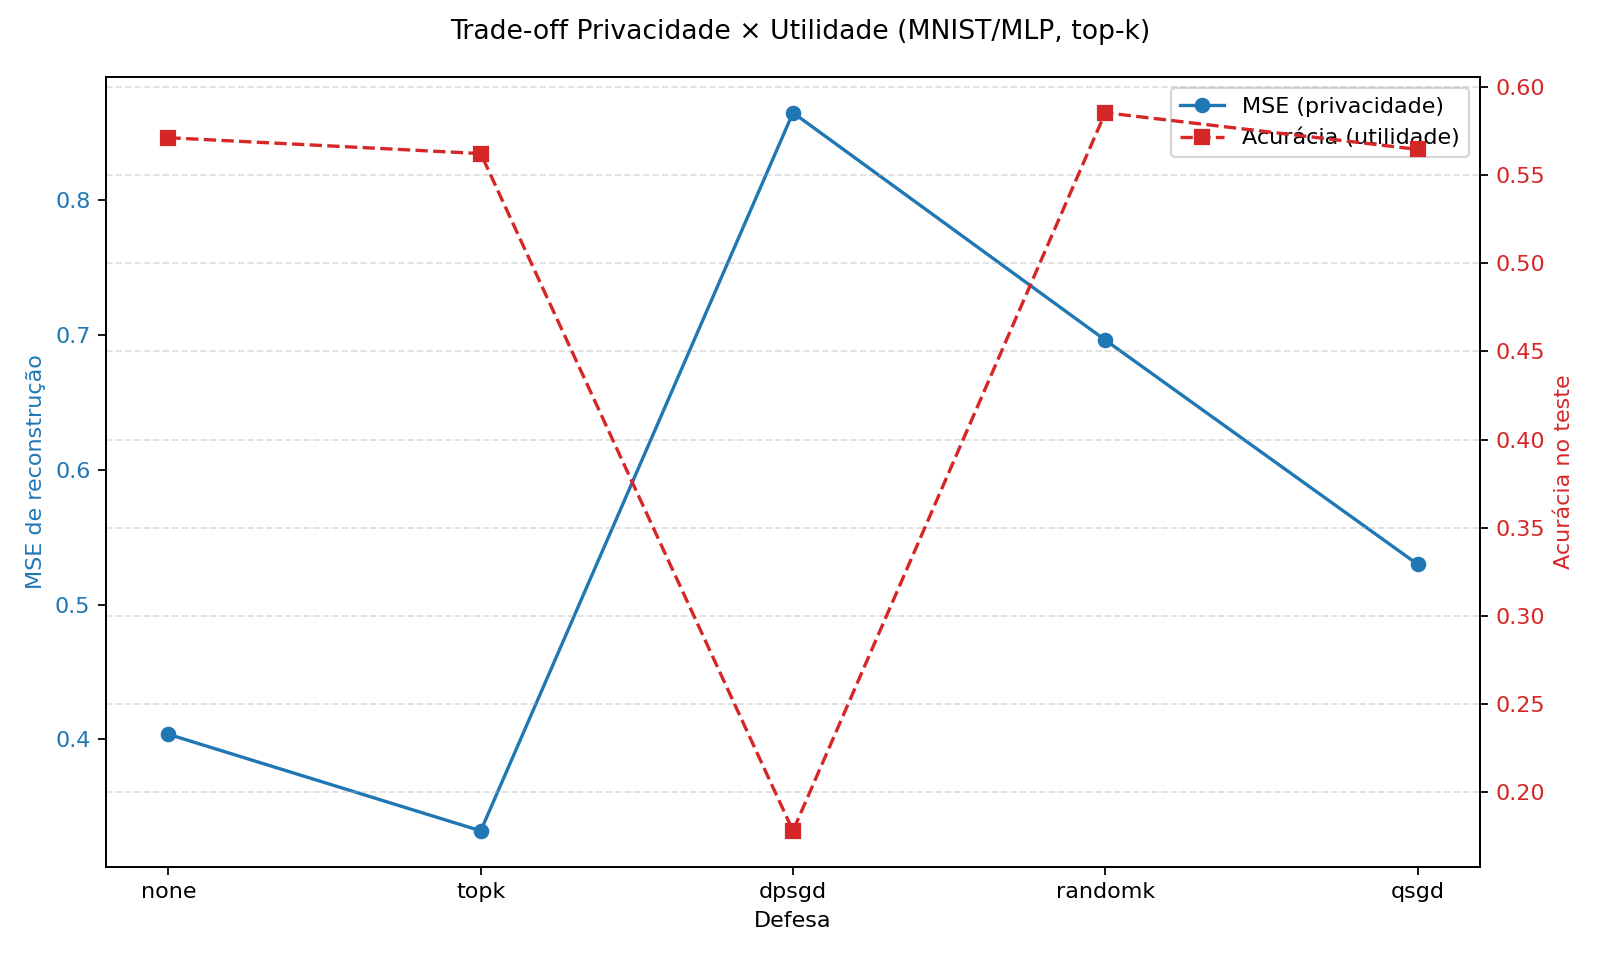
\includegraphics[width=0.88\linewidth]{../figuras_grid/tradeoff_mse_acc_global.png}
\caption{Trade-off entre MSE de reconstru\c{c}\~{a}o e acur\'{a}cia de teste (m\'{e}dias globais).}
\label{fig:tradeoff}
\end{figure}

\begin{figure}[t]
\centering
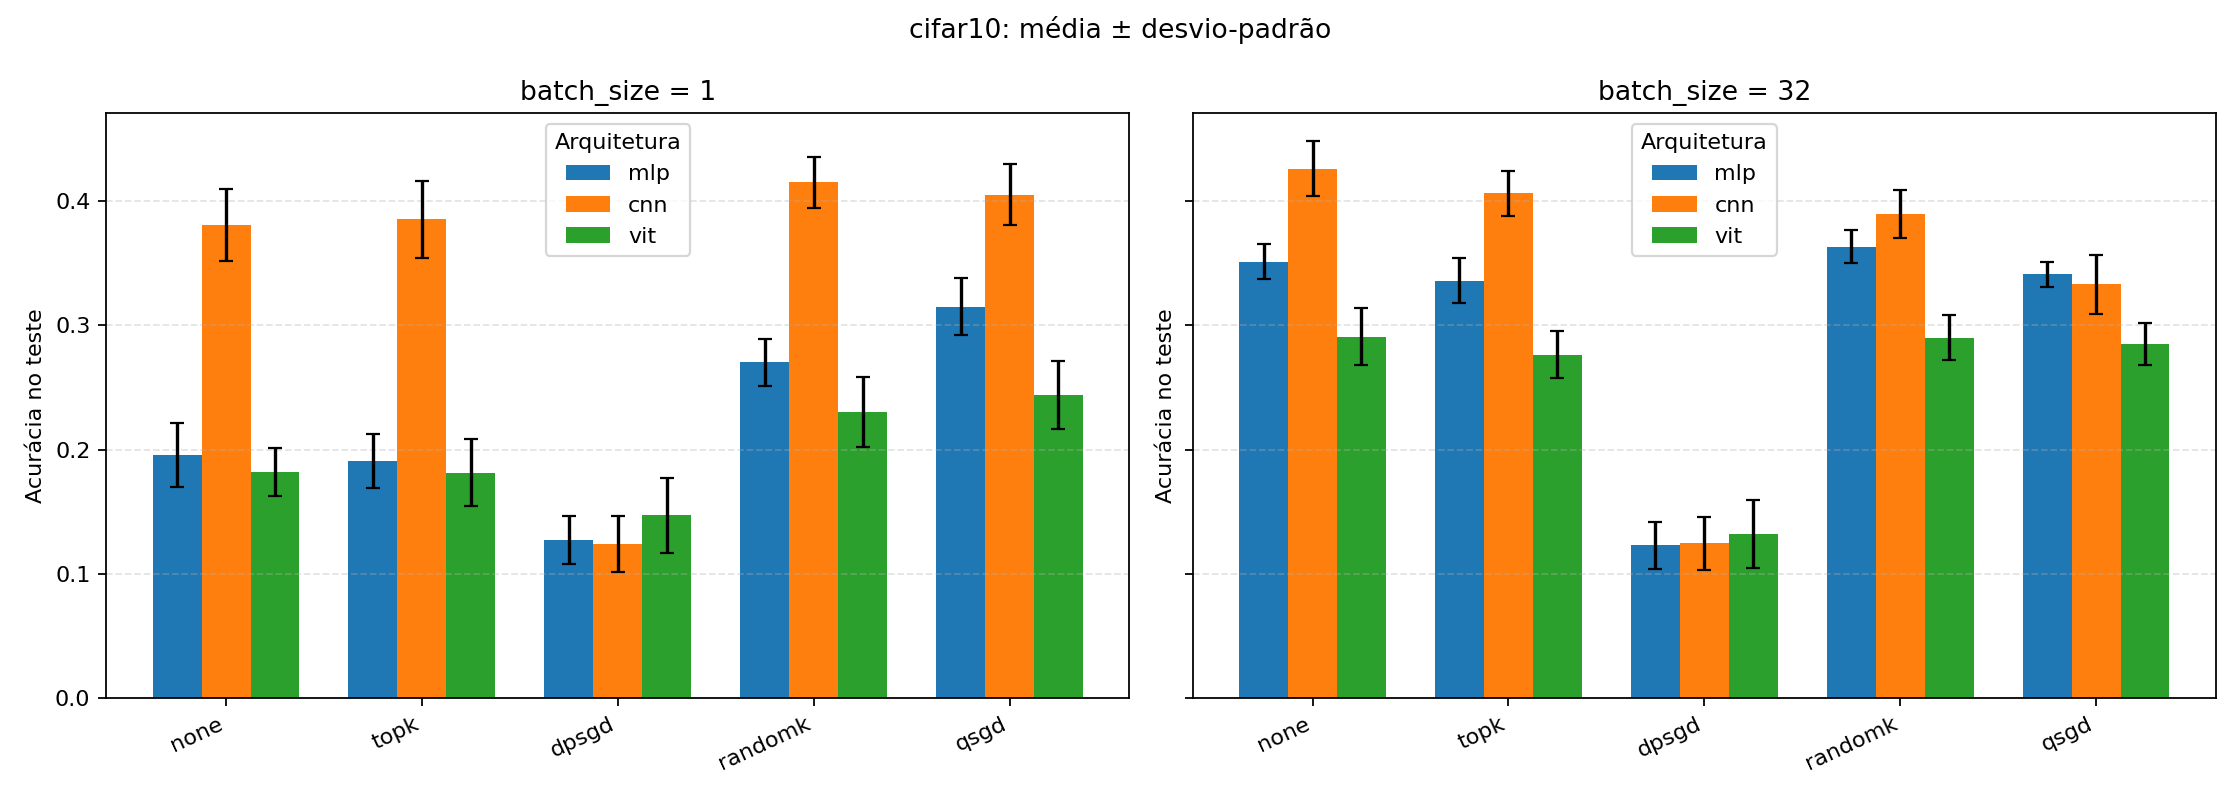
\includegraphics[width=0.88\linewidth]{../figuras_grid/acc_barras_cifar10.png}
\caption{Acur\'{a}cia de teste por defesa, arquitetura e tamanho de \textit{batch} no CIFAR-10.}
\label{fig:acc_cifar10}
\end{figure}

\subsection{Efeito da arquitetura e do tamanho de \textit{batch}}

A arquitetura modula a vulnerabilidade base e a resposta \`{a}s defesas. No CIFAR-10 sem defesa, o MSE de reconstru\c{c}\~{a}o do ViT (0,098) supera o da CNN (0,009) e do MLP (0,014), embora a acur\'{a}cia de teste do ViT (0,291) fique abaixo das demais. Random-$k$ e DP-SGD elevam o MSE do ViT para 0,303 e 0,298, respectivamente.

No CIFAR-10 com CNN, Random-$k$ constitui o melhor equil\'{\i}brio observado: MSE 9,5 vezes superior ao de \textit{none} (0,086 \textit{vs.} 0,009) e acur\'{a}cia de 0,390 (queda de 8\%). No ViT, Random-$k$ eleva o MSE de 0,098 para 0,303 com acur\'{a}cia praticamente inalterada (0,290 \textit{vs.} 0,291). O tamanho de \textit{batch} afeta predominantemente a utilidade: na CNN, aumentar o \textit{batch} de 1 para 32 eleva a acur\'{a}cia de \textit{none} de 0,381 para 0,426 ($+4{,}5$ pontos percentuais). DP-SGD permanece insens\'{\i}vel (0,124 em ambos os tamanhos). QSGD sofre maior penaliza\c{c}\~{a}o com \textit{batch}~$= 32$ (0,333 \textit{vs.} 0,405 com \textit{batch}~$= 1$).

\subsection{Resultados em MNIST e Fashion-MNIST}
\label{sec:resultados-mnist}

Em MNIST e Fashion-MNIST, a reconstru\c{c}\~{a}o sem defesa apresenta MSE elevado e alta vari\^{a}ncia, dificultando a discrimina\c{c}\~{a}o entre defesas. No MNIST com MLP, Top-$k$, Random-$k$ e QSGD produzem MSE \textit{inferior} ao de \textit{none} ($p < 0{,}05$), sugerindo que a compress\~{a}o pode facilitar inadvertidamente a otimiza\c{c}\~{a}o do ataque. Em Fashion-MNIST com CNN, Random-$k$ eleva o MSE de 0,36 para 1,59 ($p = 6{,}3 \times 10^{-10}$), enquanto Top-$k$ reduz o MSE para 0,028 ($p = 0{,}016$).

\subsection{Valida\c{c}\~{a}o da hip\'{o}tese}

A hip\'{o}tese de que mecanismos que reduzem a informa\c{c}\~{a}o nos gradientes elevam o MSE de reconstru\c{c}\~{a}o \'{e} \textbf{confirmada parcialmente}. DP-SGD, Random-$k$ e QSGD aumentam significativamente o MSE no CIFAR-10 em pelo menos duas arquiteturas, com trade-offs distintos sobre a acur\'{a}cia. Top-$k$, contudo, \textbf{n\~{a}o confirma} a hip\'{o}tese no protocolo empregado: a reten\c{c}\~{a}o de 10\% dos componentes de maior magnitude n\~{a}o impede o iDLG de inferir r\'{o}tulos com 100\% de acerto. A utilidade do modelo decresce de forma previs\'{\i}vel apenas para DP-SGD (queda de $\approx$75\%) e, em menor grau, para QSGD ($\approx$11\%) e Random-$k$ ($\approx$4\% em m\'{e}dia global).

% =============================================================================
% SE\c{C}\~{A}O 5 --- CONCLUS\~{O}ES
% =============================================================================
\section{Conclus\~{o}es}
\label{sec:conclusoes}

Este estudo comparou empiricamente cinco mecanismos de defesa contra invers\~{a}o de gradientes em um protocolo fatorial uniforme. Os resultados quantificam o trade-off entre privacidade --- medida por MSE de reconstru\c{c}\~{a}o e acerto de r\'{o}tulo via iDLG --- e utilidade --- medida por acur\'{a}cia de teste ap\'{o}s uma \'{e}poca de treinamento.

DP-SGD produziu a maior prote\c{c}\~{a}o em todas as bases e arquiteturas avaliadas, elevando o MSE m\'{e}dio global de 0,404 para 0,865 e reduzindo a acur\'{a}cia m\'{e}dia de 0,614 para 0,153. Random-$k$ emergiu como a alternativa mais equilibrada no CIFAR-10 ($p < 0{,}001$), com redu\c{c}\~{a}o de acur\'{a}cia inferior a 8\% na CNN e praticamente nula no ViT. QSGD ocupou posi\c{c}\~{a}o intermedi\'{a}ria (MSE 0,530; acur\'{a}cia 0,548). Top-$k$ a 10\% n\~{a}o diferiu estatisticamente de \textit{none} no CIFAR-10 e manteve acerto de r\'{o}tulo de 100\%. A efic\'{a}cia das defesas depende da complexidade da base de dados e da arquitetura: o CIFAR-10 permitiu discriminar os mecanismos; em MNIST, a alta vari\^{a}ncia do MSE de baseline limitou a validade comparativa. O ViT apresentou MSE base de 0,098 (CNN: 0,009; MLP: 0,014); Random-$k$ e DP-SGD elevaram o MSE para 0,303 e 0,298, respectivamente.

\subsection{Limita\c{c}\~{o}es}

O protocolo simulou um cliente \'{u}nico, sem agrega\c{c}\~{a}o multi-cliente. Empregou uma \'{u}nica \'{e}poca e subconjuntos de 4.000 amostras de treino. A avalia\c{c}\~{a}o de privacidade restringiu-se ao iDLG com L-BFGS, em \textit{checkpoints} com \textit{batch}~$= 32$; ataques adaptativos ou m\'{u}ltiplas rodadas federadas podem alterar a efic\'{a}cia relativa. Os par\^{a}metros de compress\~{a}o (10\%) e de ru\'{\i}do ($\sigma = 1{,}0$) foram fixos, sem varredura; DP-SGD n\~{a}o reportou garantia $(\varepsilon, \delta)$. Falhas de converg\^{e}ncia do ataque reduziram $n$ a 21--30 por configura\c{c}\~{a}o. Por fim, cinco de onze t\'{e}cnicas catalogadas --- LDP, RDP, SignSGD, TernGrad e DGC --- n\~{a}o foram implementadas.

\subsection{Trabalhos futuros}

Pesquisas subsequentes podem estender a grade com varredura de taxas de reten\c{c}\~{a}o, n\'{\i}veis de ru\'{\i}do e n\'{u}mero de \'{e}pocas. Podem incluir agrega\c{c}\~{a}o FedAvg, ataques adicionais (DLG, GradInversion) e t\'{e}cnicas n\~{a}o avaliadas. A combina\c{c}\~{a}o de compress\~{a}o aleat\'{o}ria com ru\'{\i}do diferencial constitui candidata natural a investiga\c{c}\~{a}o futura.

% =============================================================================
\bibliographystyle{kdmile}
\bibliography{referencias}

\begin{received}
\end{received}

\end{document}
